\documentclass{warpdoc}
\newlength\lengthfigure                  % declare a figure width unit
\setlength\lengthfigure{0.158\textwidth} % make the figure width unit scale with the textwidth
\usepackage{psfrag}         % use it to substitute a string in a eps figure
\usepackage{subfigure}
\usepackage{rotating}
\usepackage{pstricks}
\usepackage[innercaption]{sidecap} % the cute space-saving side captions
\usepackage{scalefnt}
\usepackage{amsbsy}
\usepackage{bm}
\usepackage{amsmath}
\usepackage{graphicx}

%%%%%%%%%%%%%=--NEW COMMANDS BEGINS--=%%%%%%%%%%%%%%%%%%%%%%%%%%%%%%%%%%
\newcommand{\alb}{\vspace{0.1cm}\\} % array line break
\newcommand{\rhos}{\rho}
\newcommand{\cv}{{c_v}}
\newcommand{\cp}{{c_p}}
\newcommand{\Sct}{{{\rm Sc}_{\rm T}}}
\newcommand{\Prt}{{{\rm Pr}_{\rm T}}}
\newcommand{\nd}{{{n}_{\rm d}}}
\newcommand{\ns}{{{n}_{\rm s}}}
\newcommand{\nn}{{{n}_{\rm n}}}
\newcommand{\ndm}{{\bar{n}_{\rm d}}}
\newcommand{\nsm}{{\bar{n}_{\rm s}}}
\newcommand{\turb}{_{\rm T}}
\newcommand{\mut}{{\mu\turb}}
\newcommand{\mfa}{\scriptscriptstyle}
\newcommand{\mfb}{\scriptstyle}
\newcommand{\mfc}{\textstyle}
\newcommand{\mfd}{\displaystyle}
\newcommand{\hlinex}{\vspace{-0.34cm}~~\\ \hline \vspace{-0.31cm}~~\\}
\newcommand{\hlinextop}{\vspace{-0.46cm}~~\\ \hline \hline \vspace{-0.32cm}~~\\}
\newcommand{\hlinexbot}{\vspace{-0.37cm}~~\\ \hline \hline \vspace{-0.50cm}~~\\}
\newcommand{\tablespacing}{\vspace{-0.4cm}}
\newcommand{\fontxfig}{\footnotesize\scalefont{0.918}}
\newcommand{\fontgnu}{\footnotesize\scalefont{0.896}}
\renewcommand{\fontsizetable}{\footnotesize\scalefont{1.0}}
\renewcommand{\fontsizefigure}{\footnotesize}
%\renewcommand{\vec}[1]{\pmb{#1}}
%\renewcommand{\vec}[1]{\boldsymbol{#1}}
\renewcommand{\vec}[1]{\bm{#1}}
\setcounter{tocdepth}{3}
\let\citen\cite
\newcommand\frameeqn[1]{\fbox{$\displaystyle #1$}}

%%%%%%%%%%%%%=--NEW COMMANDS BEGINS--=%%%%%%%%%%%%%%%%%%%%%%%%%%%%%%%%%%

\setcounter{tocdepth}{3}

%%%%%%%%%%%%%=--NEW COMMANDS ENDS--=%%%%%%%%%%%%%%%%%%%%%%%%%%%%%%%%%%%%



\author{
  Bernard Parent
}

\email{
  bernparent@gmail.com
}

\department{
  Institute for Aerospace Studies	
}

\institution{
  University of Toronto
}

\title{
  Thermodynamic Properties
}

\date{
  1998--2015
}

%\setlength\nomenclaturelabelwidth{0.13\hsize}  % optional, default is 0.03\hsize
%\setlength\nomenclaturecolumnsep{0.09\hsize}  % optional, default is 0.06\hsize

\nomenclature{

  \begin{nomenclaturelist}{Roman symbols}
   \item[$a$] speed of sound
  \end{nomenclaturelist}
}


\abstract{
abstract
}

\begin{document}
  \pagestyle{headings}
  \pagenumbering{arabic}
  \setcounter{page}{1}
%%  \maketitle
  \makewarpdoctitle
%  \makeabstract
  \tableofcontents
%  \makenomenclature
%%  \listoftables
%%  \listoffigures





\section{Specific heats, Enthalpies, and Entropies}

It is assumed that the mixture
is thermally perfect, but calorically imperfect. The assumption
of a thermally perfect gas has been used successfully in the
past to simulate high speed flight, and has the advantage of being
considerably easier to solve than a real gas. The reader is invited
to consult Anderson\cite{gen:anderson2} or Dudebout \cite{cfd:dudebout}
for more details.
%
\begin{table*}[ht]
  \center\fontsizetable
  \begin{threeparttable}
    \tablecaption{Constants to determine $h_k$ for some example species \tnote{a}}
    \label{table:species-real}
    \fontsizetable
    \begin{tabular*}{\textwidth}{l@{\extracolsep{\fill}}ll}
    \toprule
Species $k$                                               & ${\rm He}        $ & ${\rm H}_2        $  \\
\midrule
${\cal M}_k$       $\left[ {\rm kg}/{\rm mol} \right]$    & $+4.00260$E$-3   $ & $+2.01588000$E$-3 $  \\
    \midrule
$T_{\rm min}$     [K]                                     & $+200.0          $ & $+200.0           $  \\
$T_{\rm max}$     [K]                                     & $+1000.0         $ & $+1000.0          $   \\
$a_{1,k}$                                                 & $+2.50000000$E$+0$ & $+4.078322810$E$+4$  \\
$a_{2,k}$                                                 & $+0.00000000$E$+0$ & $-8.009185450$E$+2$   \\
$a_{3,k}$                                                 & $+0.00000000$E$+0$ & $+8.214701670$E$+0$   \\
$a_{4,k}$                                                 & $+0.00000000$E$+0$ & $-1.269714360$E$-2$   \\
$a_{5,k}$                                                 & $+0.00000000$E$+0$ & $+1.753604930$E$-5$   \\
$a_{6,k}$                                                 & $-7.45375000$E$+2$ & $-1.202860160$E$-8$   \\
$a_{7,k}$                                                 & $+9.28723974$E$-1$ & $+3.368093160$E$-12$   \\
\midrule                                
$T_{\rm min}$     [K]                                     & $+1000.0      $ & $+1000.0          $   \\
$T_{\rm max}$     [K]                                     & $+6000.0      $ & $+6000.0          $   \\
$a_{1,k}$                                                 & $+2.50000000$E$+0$ & $+5.608123380$E$+5 $   \\
$a_{2,k}$                                                 & $+0.00000000$E$+0$ & $-8.371491340$E$+2 $   \\
$a_{3,k}$                                                 & $+0.00000000$E$+0$ & $+2.975363040$E$+0 $   \\
$a_{4,k}$                                                 & $+0.00000000$E$+0$ & $+1.252249930$E$-3$  \\
$a_{5,k}$                                                 & $+0.00000000$E$+0$ & $-3.740718420$E$-7$   \\
$a_{6,k}$                                                 & $-7.45375000$E$+2$ & $+5.936628250$E$-11 $  \\
$a_{7,k}$                                                 & $+9.28723974$E$-1$ & $-3.606995730$E$-15 $   \\
            
    \bottomrule
    \end{tabular*}
    \begin{tablenotes}
      \item[a] Properties taken from McBride \cite{nasa:2002:mcbride}; {${\cal R}=8.3144126 ~~\left[ {\rm J}/{\rm mol~K} \right]$}
    \end{tablenotes}
  \end{threeparttable}
\end{table*}
%



The pressure $P$ is related to the temperature and densities 
through the equation of state
which is assumed to correspond to the one of a thermally perfect gas
using Dalton's law of partial pressures, i.e.
the pressure is the sum of the partial pressure for each species:
%
\begin{equation}
P=\sum_{k=1}^{\ns} \frac{\rho_k {\cal R} T}{{\cal M}_k}
\end{equation}
%
where ${\cal R}$ and ${\cal M}$ are tabulated for various species
in table \ref{table:species-real}. 
Let's define $R$ as the gas constant of the mixture, equal to 
$\sum w_k {\cal R} /{\cal M}_k$.
Also the enthalpy $h$, entropy $s$ and $\cp\equiv \partial h / \partial T$
are determined from a mass weighted average:
%
\begin{align}
h&=\mfd\sum_{k=1}^{\ns} w_k h_k \\
s&=\mfd\sum_{k=1}^{\ns} w_k s_k \\
\cp&=\mfd\sum_{k=1}^{\ns} w_k \cp_k 
\end{align}
%
where the species specific enthalpy, specific entropy, and specific heat at constant pressure correspond to: 
%
\begin{align}
        h_k&=\mfd\frac{\cal R}{{\cal M}_k}\left( a_{1,k} T
          + \mfd\frac{a_{2,k}}{2} T^2 + \mfd\frac{a_{3,k}}{3} T^3 + \mfd\frac{a_{4,k}}{4} T^4 + \mfd\frac{a_{5,k}}{5} T^5 + a_{6,k} \right)\\
        s_k&=\mfd\frac{\cal R}{{\cal M}_k}\left( a_{1,k} {\rm ln}(T)
          + a_{2,k} T + \mfd\frac{a_{3,k}}{2} T^2 + \mfd\frac{a_{4,k}}{3} T^3 + \mfd\frac{a_{5,k}}{4} T^4 + a_{7,k} \right) \\
        \cp_k&=\mfd\frac{\cal R}{{\cal M}_k}\left( a_{1,k}
          + a_{2,k} T + a_{3,k} T^2 + a_{4,k} T^3 + a_{5,k} T^4  \right)
\end{align}
%


Another variable needed by the primitive variables module is the static 
temperature. When dealing with a calorically imperfect gas, the static
temperature cannot be readily determined with a simple algebraic expression
from the internal energy. Solving for $T$ hence requires an iterative
process minimizing the function $\Phi(T)=e +  R T - h(T)$. 
A Newton iteration is chosen for its simplicity:
%
\begin{equation}
T^{n+1}=T^{n}-\left(\frac{\Phi} {\Phi^\prime}\right)^{n}
\end{equation}
%
where the number of steps $n$ can either be fixed to a constant (like 2 or 3)
or the iteration can be performed until acceptable accuracy is achieved.
$\Phi^\prime$ corresponds to the derivative of $\Phi$ with respect
to $T$.

Another important property to be outlined in this section is the
reference sound speed or ``thermodynamic'' sound speed $a_{\rm thermo}$:
%
\begin{equation}
a_{\rm thermo} \equiv \sqrt{\frac{R \cp T}{\cp - R}}
\end{equation}
%
It is noted that a sound speed cannot be by definition simply thermodynamic:
it must be derived from a set of governing equations including derivatives
in time and space. However, the above is commonly referred to in the
gas dynamic literature as the ``sound speed'', and for this reason is listed
here. It shall be used solely as a means to compute initial conditions in
the domain.

Further, in the determination of the linearization matrix $A$, these derivatives were needed:
%
\begin{equation}
\begin{array}{lll}
  \left. \mfd\frac{\partial e(P,\rho)}{\partial P} \right|_\rho=\mfd\frac{\cp-R}{\rho R}
  &~~~~&\left. \mfd\frac{\partial e(P,\rho)}{\partial \rho_k} \right|_{P,\rho_{\ne k}}
             =\mfd\frac{h_k-h+RT-\cp T R_k/R}{\rho} \\
~~&~~&~~\\
  \left. \mfd\frac{\partial e(T,\rho)}{\partial T} \right|_\rho=\cp-R
  &~~~~&  \left. \mfd\frac{\partial e(T,\rho)}{\partial \rho_k} \right|_{T,\rho_{\ne k}}
             =\mfd\frac{h_k-h+RT-R_k T}{\rho}
\end{array}
\end{equation}
%





\section{Properties Needed within the Vibrational and Electron Energy Transport Equations}


Also, the fraction of the Joule heating that is consumed in the excitation of the vibration levels of the nitrogen molecule, $\zeta_{\rm v}$,  is as specified in Table \ref{table:etavcoefficients}.




%
\begin{table*}
  \center\fontsizetable
  \begin{threeparttable}
    \tablecaption{Polynomial coefficients needed for the fraction of energy consumed in the excitation of vibration levels of the nitrogen molecule, $\zeta_{\rm v}=\sum_{n=0}^{10} k_n T_{\rm e}^n$.\tnote{a,b,c}} 
    \label{table:etavcoefficients}
    \fontsizetable
    \begin{tabular*}{\textwidth}{l@{\hspace{0.1\textwidth}}l}
    \toprule
      Coefficient & Value    \\
    \midrule
      $k_0$          & $\texttt{+1.8115947E-3}$   \\
      $k_1$     &  $\texttt{+2.1238526E-5}$  \\
      $k_2$ & $\texttt{-2.2082300E-8}$  \\
      $k_3$ & $\texttt{+7.3911515E-12}$  \\
      $k_4$ & $\texttt{-8.0418868E-16}$  \\
      $k_5$ & $\texttt{+4.3999729E-20}$  \\
      $k_6$ & $\texttt{-1.4009604E-24}$  \\
      $k_7$ & $\texttt{+2.7238062E-29}$  \\
      $k_8$ & $\texttt{-3.1981279E-34}$  \\
      $k_9$ & $\texttt{+2.0887979E-39}$  \\
      $k_{10}$ & $\texttt{-5.8381036E-45}$  \\
    \bottomrule
    \end{tabular*}
 \begin{tablenotes}
   \item[a] The expression for $\zeta_{\rm v}$ can be used in the range $0<T_{\rm e}<60000$~K
   \item[b] The polynomial approximates the experimental data in Ref.\ \cite{misc:1981:aleksandrov} and Ch.\ 21 of Ref.\ \citen{book:1997:grigoriev}
   \item[c] $T_{\rm e}$ is in Kelvin
 \end{tablenotes}
   \end{threeparttable}
\end{table*}
%

%
\begin{table*}
  \center\fontsizetable
  \begin{threeparttable}
    \tablecaption{Polynomial coefficients needed to determine the electron temperature, $T_{\rm e}=\max\left(T,~\exp\left(\sum_{n=0}^{8} k_n (\ln E^\star)^n\right)\right)$.\tnote{a,b,c}} 
    \label{table:Te}
    \fontsizetable
    \begin{tabular*}{\textwidth}{l@{\hspace{0.1\textwidth}}l}
    \toprule
      Coefficient & Value    \\
    \midrule
      $k_0$ & $\texttt{-3.69167532692495882511E+08}$   \\
      $k_1$ & $\texttt{-6.26956713747712671757E+07}$   \\
      $k_2$ & $\texttt{-4.65528490607805550098E+06}$   \\
      $k_3$ & $\texttt{-1.97394448288739687996E+05}$   \\
      $k_4$ & $\texttt{-5.22784662897089219769E+03}$   \\
      $k_5$ & $\texttt{-8.85545617874565635930E+01}$   \\
      $k_6$ & $\texttt{-9.36914737923363882821E-01}$   \\
      $k_7$ & $\texttt{-5.66073394421067171284E-03}$   \\
      $k_8$ & $\texttt{-1.49535882691330832494E-05}$   \\
    \bottomrule
    \end{tabular*}
 \begin{tablenotes}
   \item[a] The expression for $T_{\rm e}$ can be used in the range $0<E^\star<3\times 10^{-19}$~Vm$^2$
   \item[b] The polynomial approximates the experimental data in Ch.\ 21 of Ref.\ \citen{book:1997:grigoriev}
   \item[c] $E^\star$ is in Vm$^2$, $T_{\rm e}$ in Kelvin, $T$ in Kelvin
 \end{tablenotes}
   \end{threeparttable}
\end{table*}
%


%
\begin{table*}
  \center\fontsizetable
  \begin{threeparttable}
    \tablecaption{Electron temperature as a function of the effective electric field.\cite{misc:1981:aleksandrov}}
    \label{tab:Te}
    \fontsizetable
    \begin{tabular*}{\textwidth}{l@{\hspace{0.13\textwidth}}l@{\hspace{0.1\textwidth}}l}
    \toprule
    $|\vec{E}+\vec{V}^{\rm e} \times \vec{B}|/N_{\rm n}$ [V~m$^2$]  & $T_{\rm e}$ [eV]   &  $T_{\rm e}$ [K] \\
    \midrule
      0.1 $\times 10^{-20}$    &  0.20          &  2321.0\\
      0.2 $\times 10^{-20}$    &  0.34          &  3945.7\\
      0.3 $\times 10^{-20}$    &  0.46          &  5338.3\\
      0.4 $\times 10^{-20}$    &  0.57          &  6614.9\\
      0.5 $\times 10^{-20}$    &  0.67          &  7775.4\\
      0.6 $\times 10^{-20}$    &  0.75          &  8703.8\\
      0.8 $\times 10^{-20}$    &  0.90          & 10444.5\\
      1.0 $\times 10^{-20}$    &  0.98          & 11372.9\\
      2.0 $\times 10^{-20}$    &  1.10          & 12765.5\\
      3.0 $\times 10^{-20}$    &  1.20          & 13926.0\\
      4.0 $\times 10^{-20}$    &  1.32          & 15318.6\\
      5.0 $\times 10^{-20}$    &  1.46          & 16943.3\\
      6.0 $\times 10^{-20}$    &  1.67          & 19380.4\\
      8.0 $\times 10^{-20}$    &  2.02          & 23442.1\\
     10.0 $\times 10^{-20}$    &  2.40          & 27852.0\\
     20.0 $\times 10^{-20}$    &  4.00          & 46420.0\\
    \bottomrule
    \end{tabular*}
   \end{threeparttable}
\end{table*}
%

%
\begin{table*}
  \center\fontsizetable
  \begin{threeparttable}
    \tablecaption{Electron temperature as a function of the effective electric field as taken from Ch.\ 21 of Ref.\ \citen{book:1997:grigoriev}.}
    \label{tab:Te2}
    \fontsizetable
    \begin{tabular*}{\textwidth}{l@{\extracolsep{\fill}}llll}
    \toprule
    {$|\vec{E}+\vec{V}^{\rm e} \times \vec{B}|/N_{\rm n}$ [V~m$^2$]}  & {$(T_{\rm e})_{\rm N_2}$ [eV]} & {$(T_{\rm e})_{\rm O_2}$ [eV]} & {$T_{\rm e}$ [eV]} &  {$T_{\rm e}$ [K]} \\
    \midrule
      0.003 $\times 10^{-20}$  &  0.028  &  --  &  0.02471       &  286.8\\
      0.005 $\times 10^{-20}$  &  0.031  &  --  &  0.02736       &  317.5\\
      0.007 $\times 10^{-20}$  &  0.035  &  --  &  0.03089       &  358.5\\
      0.01 $\times 10^{-20}$   &  0.042  &  --  &  0.03707       &  430.2\\
      0.03 $\times 10^{-20}$   &  0.10   &  --  &  0.08825       & 1024.1\\
      0.05 $\times 10^{-20}$   &  0.16   &  --  &  0.1412        & 1638.6\\
      0.07 $\times 10^{-20}$   &  0.20   &  --  &  0.1765        & 2048.3\\
      0.1 $\times 10^{-20}$    &  0.28   &  0.14                    &  0.2470        & 2866.4\\
      0.3 $\times 10^{-20}$    &  0.61   &  0.30                    &  0.5371        & 6233.0\\
      0.5 $\times 10^{-20}$    &  0.74   &  0.49                    &  0.6813        & 7906.5\\
      0.7 $\times 10^{-20}$    &  0.84   &  0.73                    &  0.8142        & 9448.8\\
      1.0 $\times 10^{-20}$    &  0.93   &  1.1                     &  0.9700        &11256.9\\
      3.0 $\times 10^{-20}$    &  1.20   &  2.4                     &  1.4820        &17198.6\\
      5.0 $\times 10^{-20}$    &  1.40   &  2.9                     &  1.7525        &20337.8\\
      7.0 $\times 10^{-20}$    &  1.50   &  3.0                     &  1.8525        &21498.3\\
     10.0 $\times 10^{-20}$    &  1.90   &  3.4                     &  2.2525        &26140.3\\
     20.0 $\times 10^{-20}$    &  3.40   &  --  &  4.0392        &46874.9\\
     30.0 $\times 10^{-20}$    &  4.20   &  --  &  4.9896        &57904.3\\
    \bottomrule
    \end{tabular*}
   \end{threeparttable}
\end{table*}
%



The electron temperature needed to obtain the mobility, the effective pressure, the specific enthalpy, and the specific internal energy of the electron species is here obtained through the ``local approximation'' by assuming that the electron temperature is a function of the local reduced electric field and does not depend on its gradients in space or time. This can be shown to yield an expression for  $T_{\rm e}$ function of $E^\star$, as tabulated in Table \ref{table:Te}.  This is generally accepted to yield a good approximation of the electron temperature except within the cathode sheath. Such is not a cause of concern, however, because the latter is primarily ion dominated and does not depend significantly on electron temperature for many problems of interest.  

It is preferred to use polynomials fits to find $\zeta_{\rm v}$ and $T_{\rm e}$ rather than interpolate through the raw data directly as was done in previous simulations of weakly-ionized plasmas (see raw data in Tables \ref{tab:Te} and \ref{tab:Te2}). Using either strategy would yield similar results when using explicit schemes to integrate the governing equations. However, when using an implicit scheme as done herein, it is important to use smooth polynomials to obtain optimal convergence rates. Should we interpolate through the raw data instead of using polynomials, the derivatives within the Jacobians could change abruptly from one time step to the other and this could lead to slower convergence or even convergence hangs.




\section{Two-term solution of the Boltzmann equation using BOLSIG+}

Electron impact involves the collision of an electron with (in this case neutral) atoms or molecules. If such an event takes place, this can lead to ionization, excited states and/or electron attachment processes. Also of interest are properties derived from an electron impact process such as the reduced electric field as a function of electron energy, and derived transport coefficients and reaction rates. To compute these properties it is necessary to first obtain the electron energy distribution function (EEDF), which under the conditions of a weakly-ionized plasma cannot be assumed to follow a Maxwellian distribution. To this end, the Boltzmann solver BOLSIG+ is used to obtain such distribution function and all derived transport and rate coefficients. This solver takes as input the cross-sections in $\rm m^2$ given as a function of the energy in eV and obtains the EEDF using a two-term approximation to this distribution.

\subsection{Settings: Physics}

The following parameters are selected in the BOLSIG+ interface:

\begin{itemize}
\item[1.]{AC field: NO}
\item[2.]{$E\times B$ field: NO}
\item[3.]{Superelastics: YES}
\item[4.]{electron-electron collisions: NO}
\item[5.]{electron-ion collisions: NO}
\item[6.]{Gas/excited states temperature: 300 K}
\end{itemize}
Changes to the latter 3 paramaters do not alter the results for $E/N$ vs electron temperature for the mixtures considered herein.

\subsection{Settings: Numerics}

The number of energy intervals is set to 200 with Automatic Grid type. All remaining convergence settings are kept to defaults.

\subsection{Settings: Advanced}

The following parameters are selected in the BOLSIG+ interface:

\begin{itemize}
\item[1.]{Include electron-neutral effects on Coulomb logarithm : YES}
\item[2.]{Ion charge parameter Z: 1.0}
\item[3.]{Ion-neutral mass ratio: 1.0}
\end{itemize}
All remaining parameters are kept to the default value.

\section{Reduced electric field vs electron temperature for various electron-neutral mixtures}

The electron energy range in which BOLSIG+ results are valid depend on the energy range of the corresponding cross-section data. Here, only the converged runs are kept, and any results extrapolated by BOLSIG+ are discarded. For higher electron temperatures for which there is no BOLSIG+ solution, the data is extrapolated by placing a spline control point for an electron temperature of $5\cdot10^6$ K, and a corresponding $E/N$ value that reflects the trend of the converged BOLSIG+ results. This last control point can be be modified to get the desired accuracy at very high temperatures. Results for several mixtures are shown below.

%
\subsection{Atomic hydrogen ($\rm H$)}

All the processes involving cross-sections used in the BOLSIG+ calculation are given in Table \ref{tab:tableH}. The reduced electric field results are shown in Fig. \ref{fig:electronimpact_H}.

\begin{table*}[!htbp]
  \center\fontsizetable
  \begin{threeparttable}
    \tablecaption{$\rm H$ electron impact processes with available cross-section data.}
    \label{tab:tableH}
    \fontsizetable
    \begin{tabular*}{\textwidth}{l@{\extracolsep{\fill}}llll}
    \toprule
    {no.}  & {process} & {type} &  {eV range}  &  {ref.} \\
    \midrule
      1 & $\rm e^- + H \rightarrow H^+ + e^- + e^-$  &  ionization  &  13.6-800  &  \cite{lxc:2024:morgan} \\ 
        \midrule
      2 & $\rm e^- + H \rightarrow e^- + H$  &  momentum transfer   &  0-1000  & \cite{lxc:2024:morgan}\\  
        \midrule
      3 & $\rm e^- + H \rightarrow e^- + H(2p)$  &  excitation   &  10.2-1000  & \cite{lxc:2024:morgan}\\ 
      4 & $\rm e^- + H \rightarrow e^- + H(2s)$  &  excitation   &  10.2-1000  & \cite{lxc:2024:morgan}\\ 

    \bottomrule
    \end{tabular*}
   \end{threeparttable}
\end{table*}

\begin{figure}[!htbp]
\subfigure[]{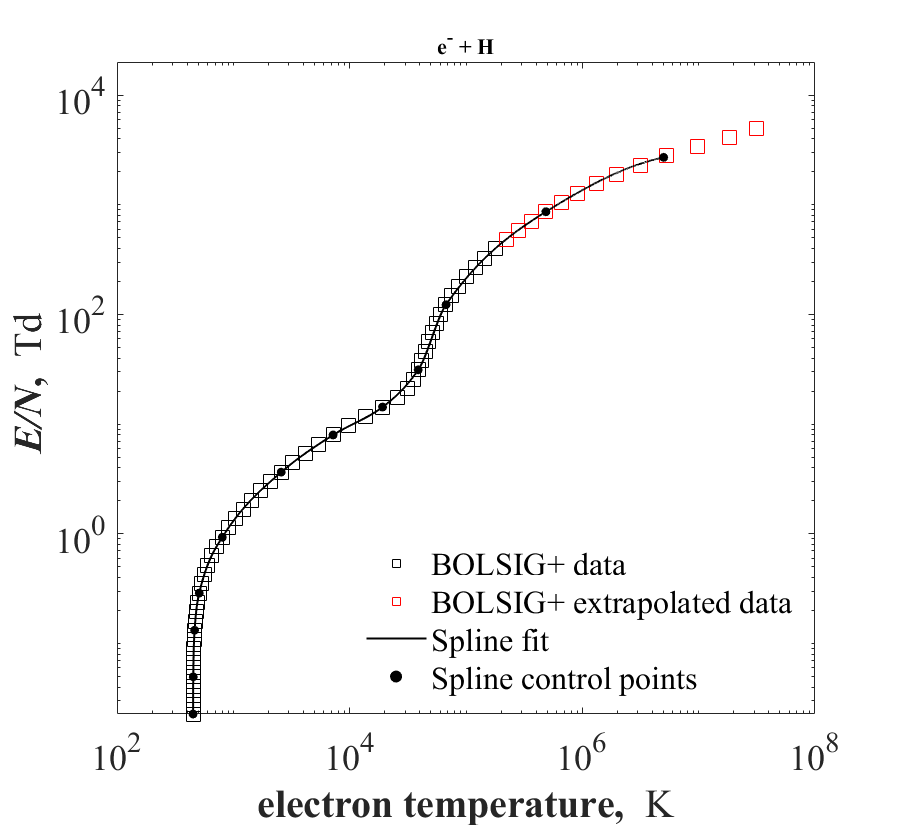
\includegraphics[width=0.99\linewidth, angle=0.0,scale=0.49]{electronimpact_figs/electronimpact_figureH.png}}
\subfigure[]{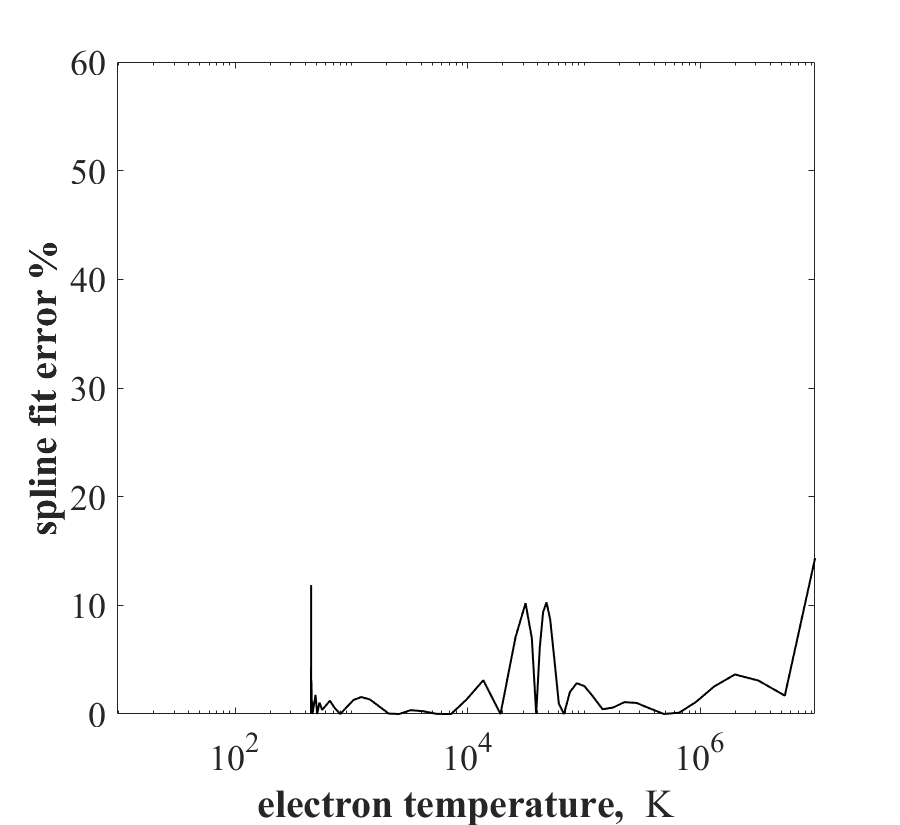
\includegraphics[width=0.99\linewidth, angle=0.0,scale=0.49]{electronimpact_figs/electronimpact_figureH_error.png}}
\caption{$E/N$ results for $\rm H$, showing (a) reduced electric field as a function of the electron temperature and (b) error percentage when fitting a cubic spline through BOLSIG+ data. The electron impact cross-sectional data used in the BOLSIG+ calculation is sourced from the Morgan database, Ref.\ \cite{lxc:2024:morgan}.}
\label{fig:electronimpact_H}
\end{figure}

%
\subsection{Hydrogen ($\rm H_2$)}

All the processes involving cross-sections used in the BOLSIG+ calculation are given in Table \ref{tab:tableH2}. The reduced electric field results are shown in Fig. \ref{fig:electronimpact_H2}.

\begin{table*}[!htbp]
  \center\fontsizetable
  \begin{threeparttable}
    \tablecaption{$\rm H_2$ electron impact processes with available cross-section data.}
    \label{tab:tableH2}
    \fontsizetable
    \begin{tabular*}{\textwidth}{l@{\extracolsep{\fill}}llll}
    \toprule
    {no.}  & {process} & {type} &  {eV range}  &  {ref.} \\
    \midrule
      1 & $\rm e^- + H_2 \rightarrow H_2^+ + e^- + e^-$  &  ionization  &  13.6-800  &  \cite{lxc:2024:morgan} \\ 
        \midrule
      2 & $\rm e^- + H_2 \rightarrow e^- + H_2$  &  momentum transfer   &  0-1000  & \cite{lxc:2024:morgan}\\  
        \midrule
      3 & $\rm e^- + H_2 \rightarrow e^- + H_2(00\rightarrow 20)$  &  rotational excitation   &  0.044-1000  & \cite{lxc:2024:morgan}\\ 
      4 & $\rm e^- + H_2 \rightarrow e^- + H_2(10\rightarrow 30)$  &  rotational excitation   &  0.079-1000  & \cite{lxc:2024:morgan}\\ 
              \midrule
      5 & $\rm e^- + H_2 \rightarrow e^- + H_2$$(\nu_1)$  &  vibrational excitation   &  0.516-1000  & \cite{lxc:2024:morgan}\\
      6 & $\rm e^- + H_2 \rightarrow e^- + H_2$$(\nu_2)$  &  vibrational excitation   &  1.000-1000  & \cite{lxc:2024:morgan}\\
      7 & $\rm e^- + H_2 \rightarrow e^- + H_2$$(\nu_3)$  &  vibrational excitation   &  1.500-1000  & \cite{lxc:2024:morgan}\\
                    \midrule
      8 & $\rm e^- + H_2 \rightarrow e^- + H_2$$(B^3\Sigma)$  &  electronic excitation   &  8.900-1000  & \cite{lxc:2024:morgan}\\
      9 & $\rm e^- + H_2 \rightarrow e^- + H_2$$(B^1\Sigma)$  &  electronic excitation   &  11.30-1000  & \cite{lxc:2024:morgan}\\
      10 & $\rm e^- + H_2 \rightarrow e^- + H_2$$(C^3\Pi)$  &  electronic excitation   &  11.75-1000  & \cite{lxc:2024:morgan}\\
      11 & $\rm e^- + H_2 \rightarrow e^- + H_2$$(A^3\Sigma)$  &  electronic excitation   &  11.80-1000  & \cite{lxc:2024:morgan}\\
     12 & $\rm e^- + H_2 \rightarrow e^- + H_2$$(C^1\Pi)$  &  electronic excitation   &  12.40-1000  & \cite{lxc:2024:morgan}\\
     13 & $\rm e^- + H_2 \rightarrow e^- + H_2$$({}^1\Sigma)$  &  electronic excitation   &  13.86-1000  & \cite{lxc:2024:morgan}\\
     14 & $\rm e^- + H_2 \rightarrow e^- + H_2$$(D^3\Pi)$  &  electronic excitation   &  14.00-1000  & \cite{lxc:2024:morgan}\\
     15 & $\rm e^- + H_2 \rightarrow e^- + H_{2}^*$  &  excitation   &  15.00-1000  & \cite{lxc:2024:morgan}\\
     16 & $\rm e^- + H_2 \rightarrow e^- + H_2$(Rydberg)  &  excitation   &  15.20-1000  & \cite{lxc:2024:morgan}\\
     16 & $\rm e^- + H_2 \rightarrow e^- + H_{2}^*$  &  excitation   &  16.60-1000  & \cite{lxc:2024:morgan}\\
    \bottomrule
    \end{tabular*}
   \end{threeparttable}
\end{table*}

\begin{figure}[!htbp]
\centering
\subfigure[]{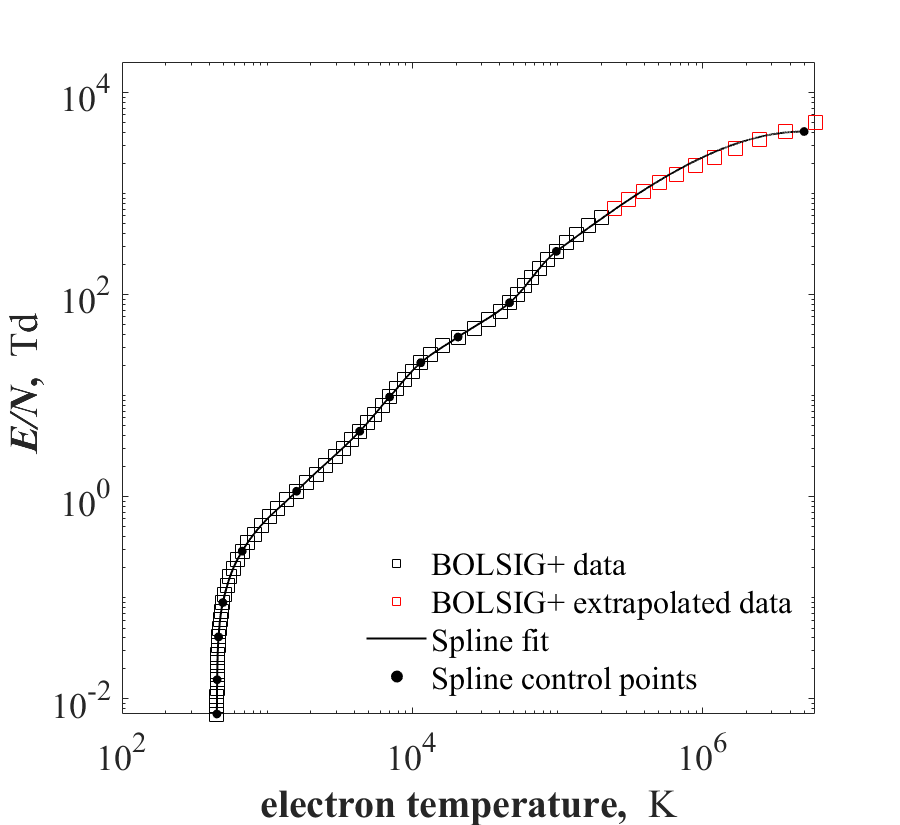
\includegraphics[width=0.99\linewidth, angle=0.0,scale=0.49]{electronimpact_figs/electronimpact_figureH2.png}}
\subfigure[]{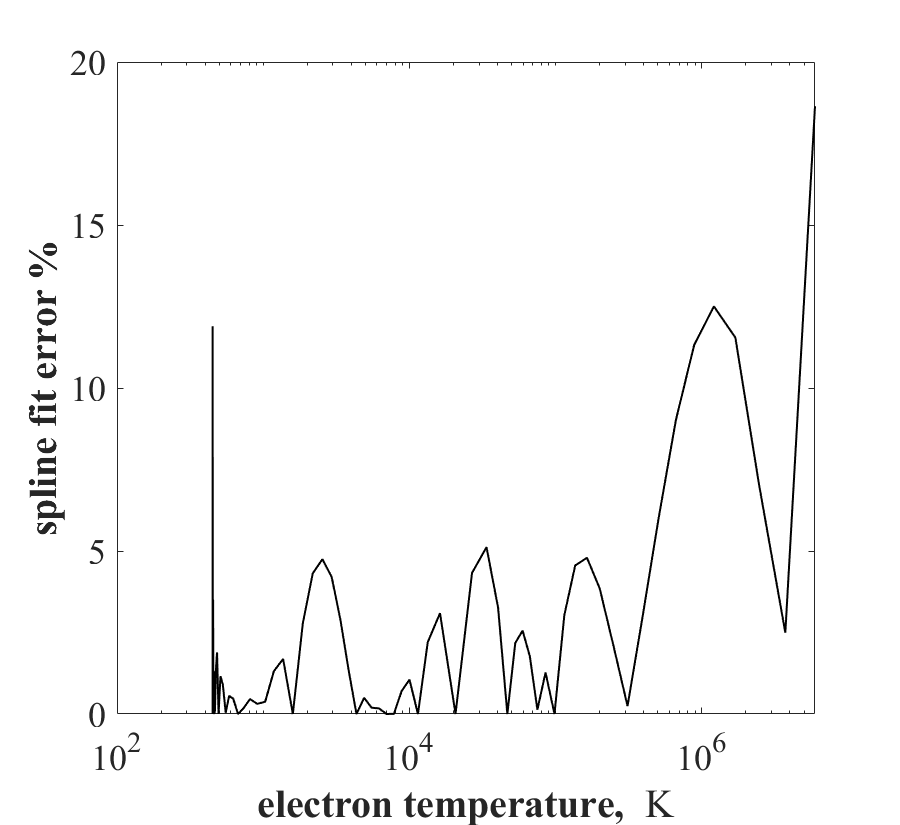
\includegraphics[width=0.99\linewidth, angle=0.0,scale=0.49]{electronimpact_figs/electronimpact_figureH2_error.png}}
\subfigure[]{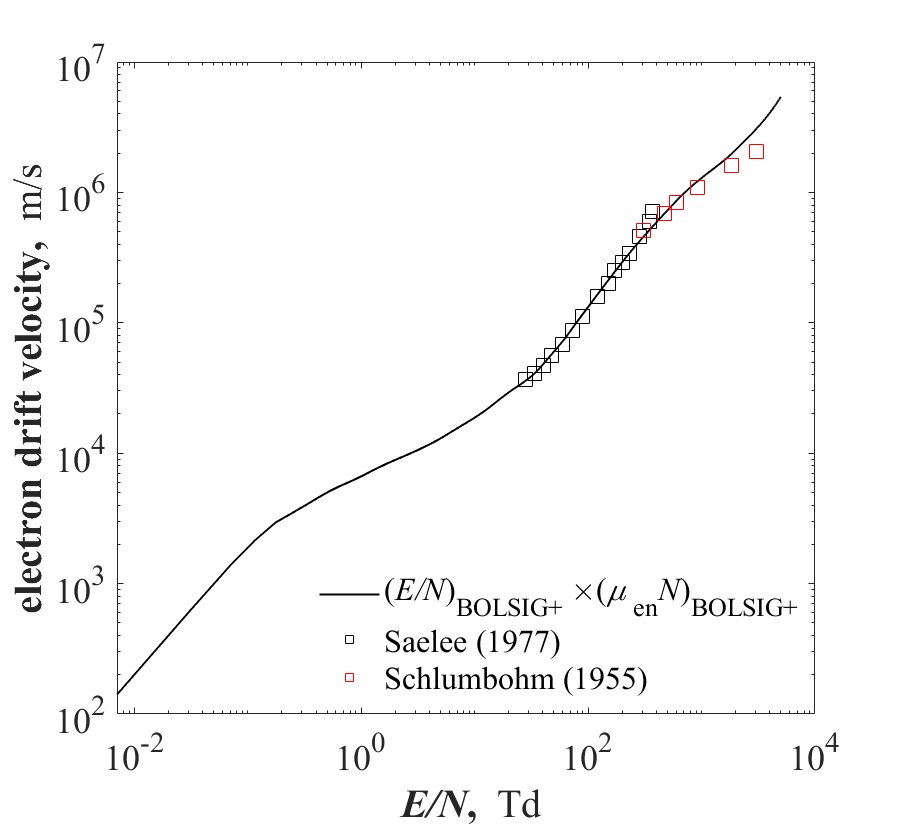
\includegraphics[width=0.99\linewidth, angle=0.0,scale=0.49]{electronimpact_figs/electronimpact_figureH2_drift.png}}
\caption{$E/N$ results for $\rm H_2$, showing (a) reduced electric field as a function of the electron temperature, (b) error percentage when fitting a cubic spline through BOLSIG+ data and c) drift velocity obtained from BOLSIG+ data as the product of the reduced electron mobility and the reduced electric field. The electron impact cross-sectional data used in the BOLSIG+ calculation is sourced from the Morgan database, Ref.\ \cite{lxc:2024:morgan}. Experimental drift velocity data is taken from Refs.\ \cite{thesis:1965:schlumbohm} and \cite{jop:1977:saelee}.}
\label{fig:electronimpact_H2}
\end{figure}
%

%
\subsection{Atomic nitrogen ($\rm N$)}

All the processes involving cross-sections used in the BOLSIG+ calculation are given in Table \ref{tab:tableN}. The reduced electric field results are shown in Fig. \ref{fig:electronimpact_4}.

\begin{table*}[!htbp]
  \center\fontsizetable
  \begin{threeparttable}
    \tablecaption{$\rm N$ electron impact processes with available cross-section data.}
    \label{tab:tableN}
    \fontsizetable
    \begin{tabular*}{\textwidth}{l@{\extracolsep{\fill}}llll}
    \toprule
    {no.}  & {process} & {type} &  {eV range}  &  {ref.} \\
    \midrule
      1 & $\rm e^- + N \rightarrow N^+ + e^- + e^-$  &  ionization   &  14.54-1000 &   \cite{lxc:2024:morgan} \\ 
      \midrule     
      2 & $\rm e^- + N \rightarrow e^- + N$  &  momentum transfer   &  0-23.1  & \cite{lxc:2024:morgan}\\   
      \midrule
      3 & $\rm e^- + N \rightarrow e^- + N(2p3)2D^0 $  &  electronic excitation   &  2.38-1000 & \cite{lxc:2024:morgan}\\ 
      4 & $\rm e^- + N \rightarrow e^- + N(2p3)2P^0 $  &  electronic excitation   &  3.58-1000 & \cite{lxc:2024:morgan}\\ 
      5 & $\rm e^- + N \rightarrow e^- + N(3p)4P $  &  electronic excitation   &  10.3-1000 & \cite{lxc:2024:morgan}\\ 
      6 & $\rm e^- + N \rightarrow e^- + N(2s2p4)4P $  &  electronic excitation   &  10.9-1000 & \cite{lxc:2024:morgan}\\ 
      7 & $\rm e^- + N \rightarrow e^- + N(3p) $  &  electronic excitation   &  11.84-1000 & \cite{lxc:2024:morgan}\\ 
      8 & $\rm e^- + N \rightarrow e^- + N(4s)4P $  &  electronic excitation   &  12.85-1000 & \cite{lxc:2024:morgan}\\ 
      9 & $\rm e^- + N \rightarrow e^- + N(3d) $  &  electronic excitation   &  13.0-1000 & \cite{lxc:2024:morgan}\\ 
      10 & $\rm e^- + N \rightarrow e^- + N(4p) $  &  electronic excitation   &  13.24-1000 & \cite{lxc:2024:morgan}\\ 
    \bottomrule
    \end{tabular*}
   \end{threeparttable}
\end{table*}

\begin{figure}[!htbp]
\subfigure[]{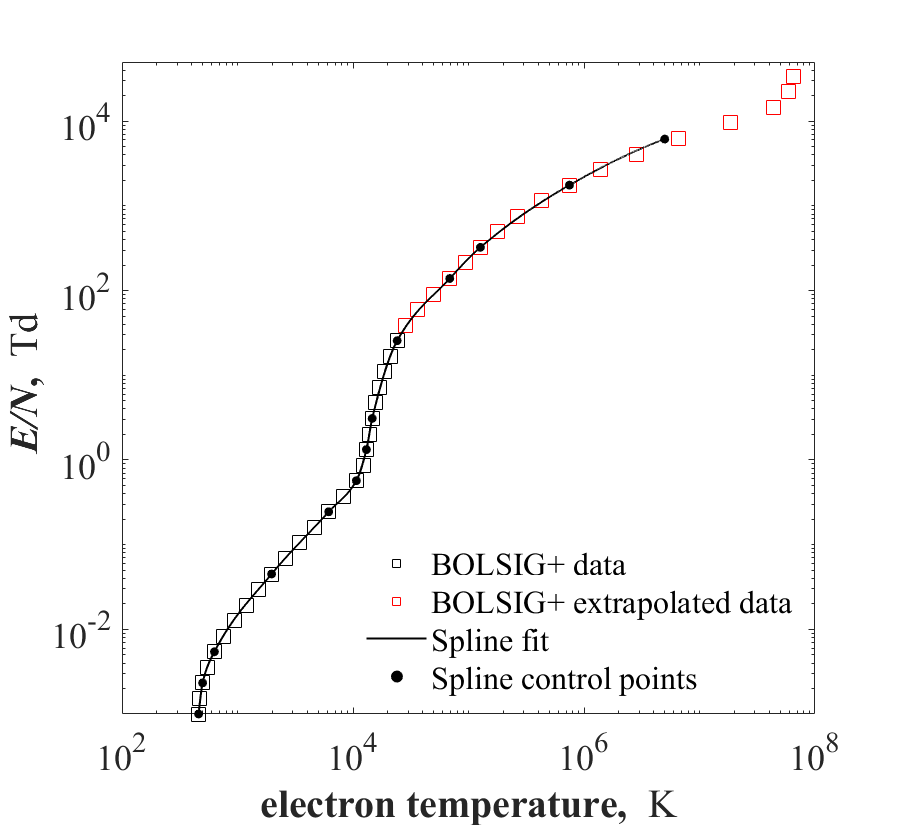
\includegraphics[width=0.99\linewidth, angle=0.0,scale=0.49]{electronimpact_figs/electronimpact_figure4.png}}
\subfigure[]{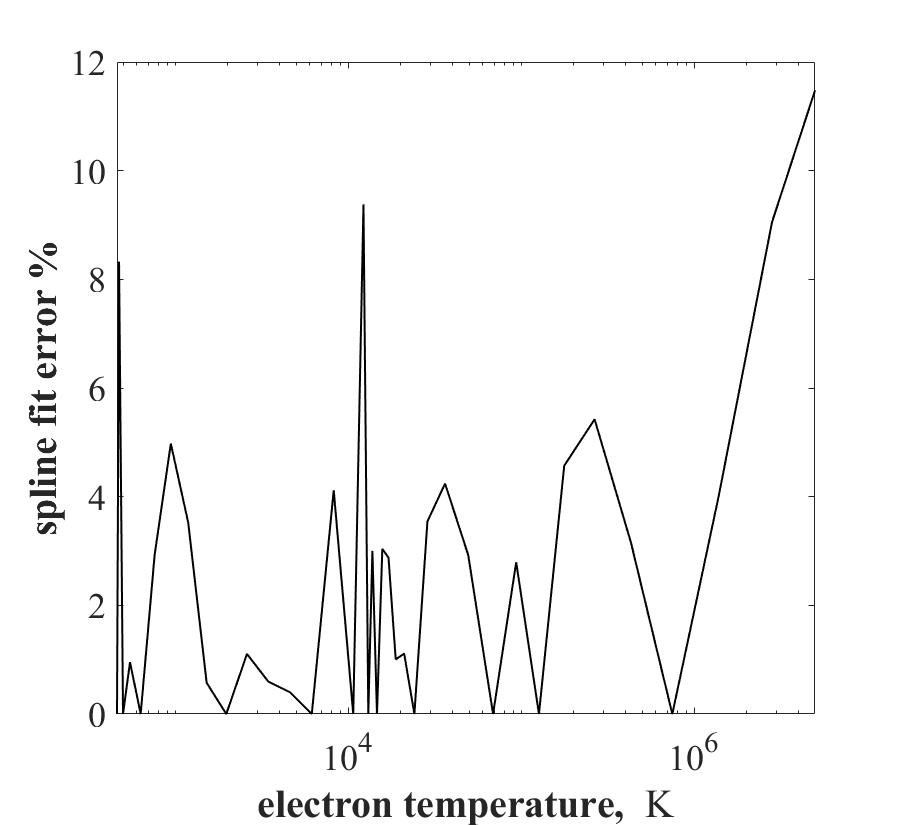
\includegraphics[width=0.99\linewidth, angle=0.0,scale=0.49]{electronimpact_figs/electronimpact_figure4_error.png}}
\caption{$E/N$ results for $\rm N$, showing (a) reduced electric field as a function of the electron temperature and (b) error percentage when fitting a cubic spline through BOLSIG+ data. The electron impact cross-sectional data used in the BOLSIG+ calculation is sourced from the Morgan database, Ref.\ \cite{lxc:2024:morgan}.}
\label{fig:electronimpact_4}
\end{figure}
%
\subsection{Atomic oxygen ($\rm O$)}

All the processes involving cross-sections used in the BOLSIG+ calculation are given in Table \ref{tab:tableO}. The reduced electric field results are shown in Fig. \ref{fig:electronimpact_5}.

\begin{table*}[!htbp]
  \center\fontsizetable
  \begin{threeparttable}
    \tablecaption{$\rm O$ electron impact processes with available cross-section data.}
    \label{tab:tableO}
    \fontsizetable
    \begin{tabular*}{\textwidth}{l@{\extracolsep{\fill}}llll}
    \toprule
    {no.}  & {process} & {type} &  {eV range}  &  {ref.} \\
    \midrule
      1 & $\rm e^- + O \rightarrow O^+ + e^- + e^-$  &  ionization   &  13.6-1000 &   \cite{lxc:2024:morgan} \\ 
      \midrule     
      2 & $\rm e^- + O \rightarrow e^- + O$  &  momentum transfer   &  0-23.1  & \cite{lxc:2024:morgan}\\   
      \midrule
      3 & $\rm e^- + O \rightarrow e^- + O(1D) $  &  electronic excitation   &  1.97-81 & \cite{lxc:2024:morgan}\\ 
      4 & $\rm e^- + O \rightarrow e^- + O(1S) $  &  electronic excitation   &  4.19-81 & \cite{lxc:2024:morgan}\\ 
    \bottomrule
    \end{tabular*}
   \end{threeparttable}
\end{table*}


\begin{figure}[!htbp]
\subfigure[]{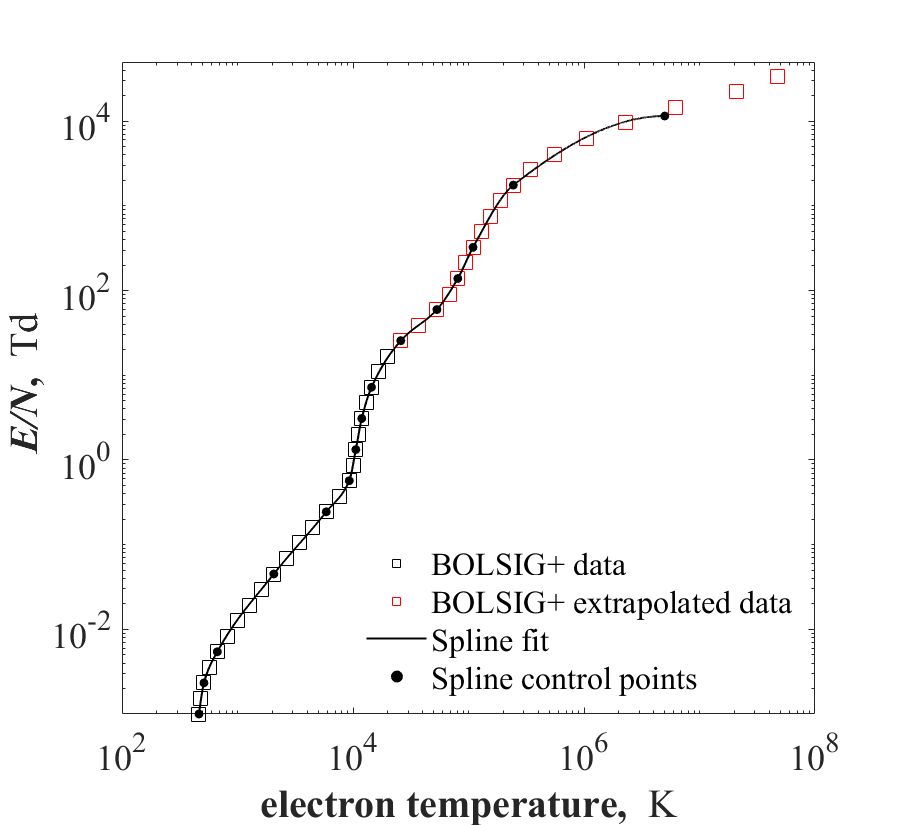
\includegraphics[width=0.99\linewidth, angle=0.0,scale=0.49]{electronimpact_figs/electronimpact_figure5.png}}
\subfigure[]{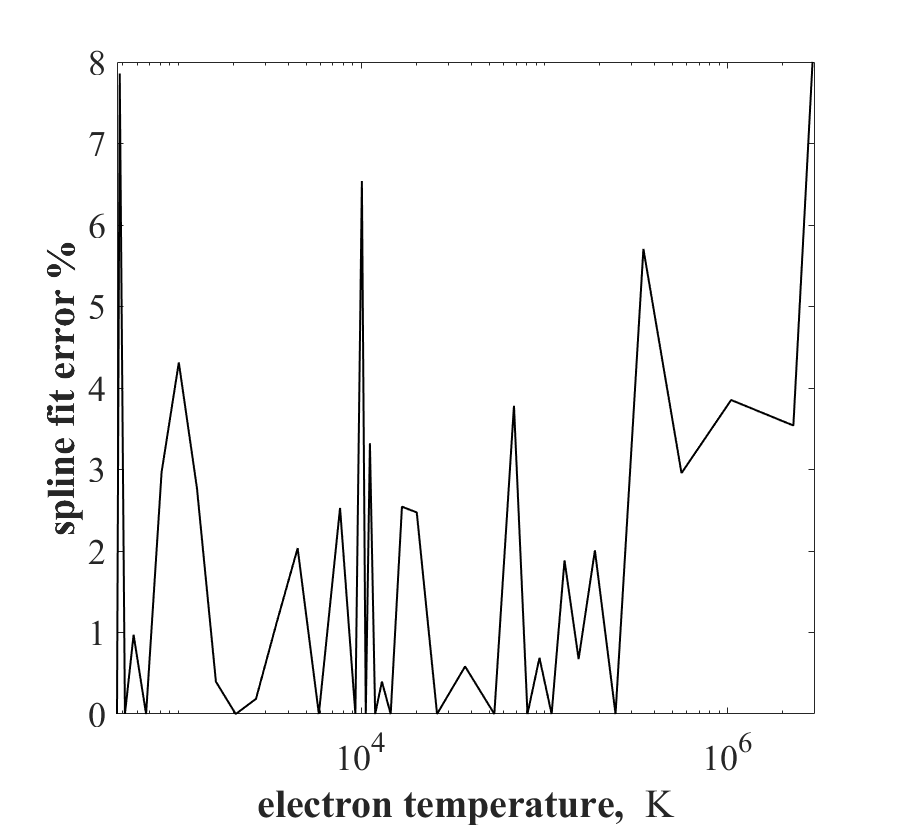
\includegraphics[width=0.99\linewidth, angle=0.0,scale=0.49]{electronimpact_figs/electronimpact_figure5_error.png}}
\caption{$E/N$ results for $\rm O$, showing (a) reduced electric field as a function of the electron temperature and (b) error percentage when fitting a cubic spline through BOLSIG+ data. The electron impact cross-sectional data used in the BOLSIG+ calculation is sourced from the Morgan database, Ref.\ \cite{lxc:2024:morgan}.}
\label{fig:electronimpact_5}
\end{figure}
%

\subsection{Nitrogen molecule ($\rm N_2$)}

Experimental data for $E/N$ vs electron temperature is available from Ch.\ 21 of Ref.\ \citen{book:1997:grigoriev} for $\rm N_2$. In this case a cubic spline is fitted through the experimental data points and also through the remaining lower and upper ranges, if any, for which there is BOLSIG+ data. All the processes involving cross-sections used in the BOLSIG+ calculation are given in Table \ref{tab:tableN2}. The reduced electric field results are shown in Fig. \ref{fig:electronimpact_1}. 

\begin{table*}[!htbp]
  \center\fontsizetable
  \begin{threeparttable}
    \tablecaption{$\rm N_2$ electron impact processes with available cross-section data.}
    \label{tab:tableN2}
    \fontsizetable
    \begin{tabular*}{\textwidth}{l@{\extracolsep{\fill}}llll}
    \toprule
    {no.}  & {process} & {type} &  {eV range}  &  {ref.} \\
    \midrule
      1 & $\rm e^- + N_2 \rightarrow N_2^+ + e^- + e^-$  &  ionization    &  15.6-1500 &   \cite{lxc:2024:morgan} \\ 
      \midrule     
      2 & $\rm e^- + N_2 \rightarrow e^- + N_2$  &  momentum transfer   &  0-1000  & \cite{lxc:2024:morgan}\\   
      \midrule
      3 & $\rm e^- + N_2 \rightarrow e^- + N_2^* $  &  rotational excitation   &  0.02-35 & \cite{lxc:2024:morgan}\\ 
           \midrule
      4 & $\rm e^- + N_2 \rightarrow e^- + N_2$$(\nu_1)$  &  vibrational excitation   &  0.290-35 &\cite{lxc:2024:morgan}\\  
      5 & $\rm e^- + N_2 \rightarrow e^- + N_2$$(\nu_1)$  &  vibrational excitation   &  0.291-35 &\cite{lxc:2024:morgan}\\  
      6 & $\rm e^- + N_2 \rightarrow e^- + N_2$$(\nu_2)$  &  vibrational excitation   &  0.590-35 &\cite{lxc:2024:morgan}\\ 
      7 & $\rm e^- + N_2 \rightarrow e^- + N_2$$(\nu_3)$  &  vibrational excitation   &  0.880-35 &\cite{lxc:2024:morgan}\\ 
      8 & $\rm e^- + N_2 \rightarrow e^- + N_2$$(\nu_4)$  &  vibrational excitation   &  1.170-35 &\cite{lxc:2024:morgan}\\ 
      9 & $\rm e^- + N_2 \rightarrow e^- + N_2$$(\nu_5)$  &  vibrational excitation   &  1.470-35 &\cite{lxc:2024:morgan}\\
      10 & $\rm e^- + N_2 \rightarrow e^- + N_2$$(\nu_6)$  &  vibrational excitation   &  1.760-35 &\cite{lxc:2024:morgan}\\ 
      11 & $\rm e^- + N_2 \rightarrow e^- + N_2$$(\nu_7)$  &  vibrational excitation   &  2.060-35 &\cite{lxc:2024:morgan}\\ 
      12 & $\rm e^- + N_2 \rightarrow e^- + N_2$$(\nu_8)$  &  vibrational excitation   &  2.350-35 &\cite{lxc:2024:morgan}\\ 
          \midrule
      13 & $\rm e^- + N_2 \rightarrow e^- + N_2$$(A^3 \Sigma_{u}^+) $  &  electronic excitation   &  6.170-35 & \cite{lxc:2024:morgan}\\ 
      14 & $\rm e^- + N_2 \rightarrow e^- + N_2$$(A^3 \Sigma_{u}^+)$  &  electronic excitation   &  7.000-35 & \cite{lxc:2024:morgan}\\ 
      15 & $\rm e^- + N_2 \rightarrow e^- + N_2$$(B^3 \Pi_{g}) $  &  electronic excitation   &  7.350-35 & \cite{lxc:2024:morgan}\\ 
      16 & $\rm e^- + N_2 \rightarrow e^- + N_2$$(W^3 \Delta) $  &  electronic excitation   &  7.360-35 & \cite{lxc:2024:morgan}\\ 
      17 & $\rm e^- + N_2 \rightarrow e^- + N_2$$(A^3 \Sigma_{u}^+) $  &  electronic excitation   &  7.80-35 & \cite{lxc:2024:morgan}\\ 
      18 & $\rm e^- + N_2 \rightarrow e^- + N_2$$(B^3 \Sigma) $  &  electronic excitation   &  8.16-35 & \cite{lxc:2024:morgan}\\ 
      19 & $\rm e^- + N_2 \rightarrow e^- + N_2$$(A^1 \Sigma) $  &  electronic excitation   &  8.40-35 & \cite{lxc:2024:morgan}\\ 
      20 & $\rm e^- + N_2 \rightarrow e^- + N_2$$(A^1 \Pi) $  &  electronic excitation   &  8.55-35 & \cite{lxc:2024:morgan}\\ 
      21 & $\rm e^- + N_2 \rightarrow e^- + N_2$$(W^1 \Delta) $  &  electronic excitation   &  8.89-35 & \cite{lxc:2024:morgan}\\ 
      22 & $\rm e^- + N_2 \rightarrow e^- + N_2$$(C^3 \Pi) $  &  electronic excitation   &  11.03-35 & \cite{lxc:2024:morgan}\\ 
      23 & $\rm e^- + N_2 \rightarrow e^- + N_2$$(E^3 \Sigma) $  &  electronic excitation   &  11.88-35 & \cite{lxc:2024:morgan}\\  
      24 & $\rm e^- + N_2 \rightarrow e^- + N_2$$(A^1 \Sigma) $  &  electronic excitation   &  12.25-35 & \cite{lxc:2024:morgan}\\ 
      25 & $\rm e^- + N_2 \rightarrow e^- + N + N $  &  electronic excitation   &  13.00-35 & \cite{lxc:2024:morgan}\\ 
    \bottomrule
    \end{tabular*}
   \end{threeparttable}
\end{table*}

\begin{figure}[!htbp]
\subfigure[]{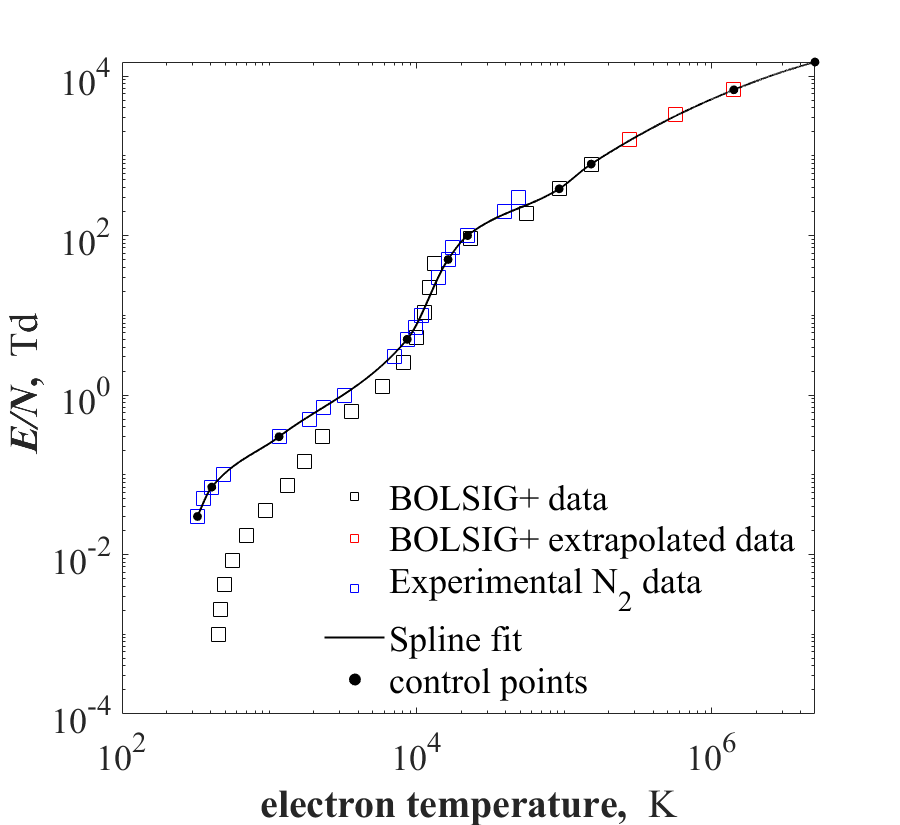
\includegraphics[width=0.99\linewidth, angle=0.0,scale=0.49]{electronimpact_figs/electronimpact_figure1.png}}
\subfigure[]{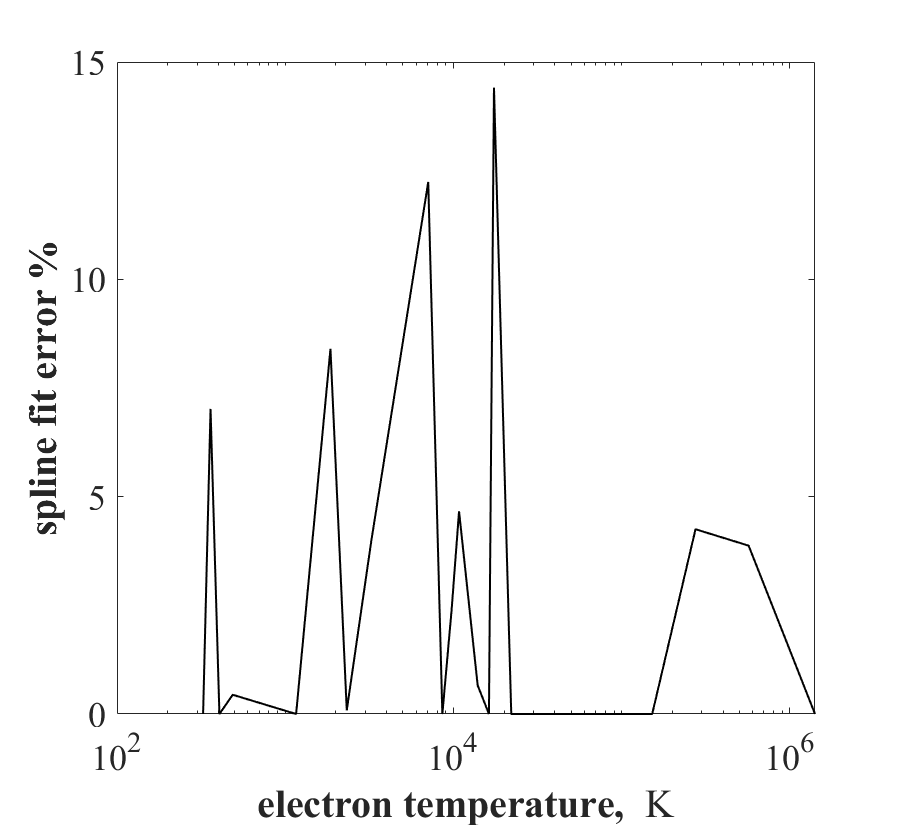
\includegraphics[width=0.99\linewidth, angle=0.0,scale=0.49]{electronimpact_figs/electronimpact_figure1_error.png}}
\caption{$E/N$ results for $\rm N_2$, showing (a) reduced electric field as a function of the electron temperature and (b) error percentage when fitting a cubic spline through the data. Experimental $\rm N_2$ data points are taken from Ref.\ \citen{book:1997:grigoriev}.}
\label{fig:electronimpact_1}
\end{figure}
%
\subsection{Oxygen molecule ($\rm O_2$)}

All the processes involving cross-sections used in the BOLSIG+ calculation are given in Table \ref{tab:tableO2}. Experimental data for $E/N$ vs electron temperature is available from Ch.\ 21 of Ref.\ \citen{book:1997:grigoriev} for $\rm O_2$. A cubic spline is fitted through the experimental data points and also through the remaining lower and upper ranges, if any, for which there is BOLSIG+ data.  The reduced electric field results are shown in Fig. \ref{fig:electronimpact_2}. In this case, no experimental data is available for $T_{\rm e}<1000$ K. Rather than make use of the BOLSIG+ results at low electron temperature which might not be accurate, we here prefer to extrapolate from the experimental data to lower $T_{\rm e}$. To do this, the experimental results for air are used and the corresponding $E/N$ value is obtained by summing the $\rm N_2$, $\rm O_2$ $E/N$ results weighed by their corresponding composition in dry air. The extrapolation of the $\rm O_2$ curve for $T_{\rm e}<1000$ K is such that there is good agreement between the experimental data and spline curve fit for air. The latter is shown in Fig. \ref{fig:electronimpact_2}. All the processes involving cross-sections used in the BOLSIG+ calculation are given in Table \ref{tab:tableO2}.
%



\begin{table*}[!htbp]
  \center\fontsizetable
  \begin{threeparttable}
    \tablecaption{$\rm O_2$ electron impact processes with available cross-section data.}
    \label{tab:tableO2}
    \fontsizetable
    \begin{tabular*}{\textwidth}{l@{\extracolsep{\fill}}llll}
    \toprule
    {no.}  & {process} & {type} &  {eV range}  &  {ref.} \\
    \midrule
      1 & $\rm e^- + O_2 \rightarrow O_2^+ + e^- + e^-$  &  ionization   &  12.6-1500 &   \cite{lxc:2024:morgan} \\ 
      \midrule     
      2 & $\rm e^- + O_2 \rightarrow e^- + O_2$  &  momentum transfer   &  0-1000  & \cite{lxc:2024:morgan}\\   
      \midrule
      3 & $\rm e^- + O_2 \rightarrow e^- + O_2^* $  &  rotational excitation   &  0.38-20 & \cite{lxc:2024:morgan}\\ 
           \midrule
      4 & $\rm e^- + O_2 \rightarrow e^- + O_2$$(\nu_1) $  &  vibrational excitation   &  0.57-15 &\cite{lxc:2024:morgan}\\  
      5 & $\rm e^- + O_2 \rightarrow e^- + O_2$$(\nu_2) $  &  vibrational excitation   &  0.75-15 &\cite{lxc:2024:morgan}\\ 
          \midrule
      6 & $\rm e^- + O_2 \rightarrow e^- + O_2$$(A^1 \Delta) $  &  electronic excitation   &  0.977-45 & \cite{lxc:2024:morgan}\\ 
      7 & $\rm e^- + O_2 \rightarrow e^- + O_2$$(B^1 \Sigma) $  &  electronic excitation   &  1.627-45 & \cite{lxc:2024:morgan}\\ 
      8 & $\rm e^- + O_2 \rightarrow e^- + O_2(-) $  &  electronic excitation   &  4.50-45 & \cite{lxc:2024:morgan}\\ 
      9 & $\rm e^- + O_2 \rightarrow e^- + O_2(-) $  &  electronic excitation   &  6.00-45 & \cite{lxc:2024:morgan}\\ 
      10 & $\rm e^- + O_2 \rightarrow e^- + O_2(-) $  &  electronic excitation   &  8.40-45 & \cite{lxc:2024:morgan}\\ 
      11 & $\rm e^- + O_2 \rightarrow e^- + O_2(-) $  &  electronic excitation   &  9.97-100 & \cite{lxc:2024:morgan}\\ 
      12 & $\rm e^- + O_2 \rightarrow e^- + O + O $  &  electronic excitation   &  14.70-100 & \cite{lxc:2024:morgan}\\ 
    \bottomrule
    \end{tabular*}

   \end{threeparttable}
\end{table*}
%
\begin{figure}[!htbp]
\subfigure[]{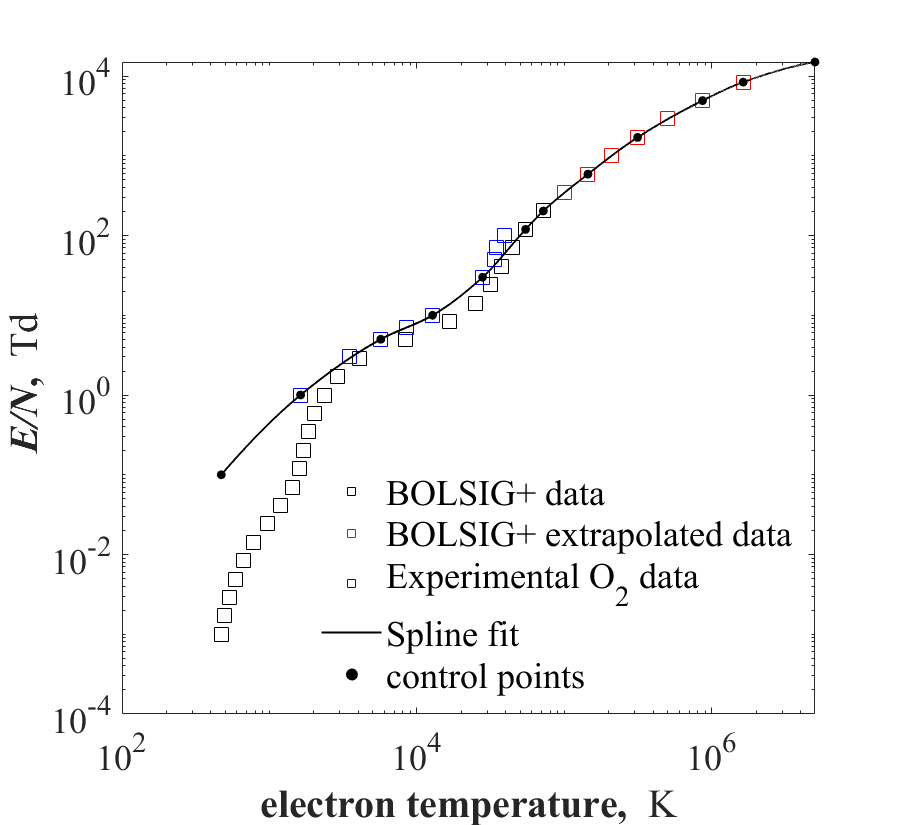
\includegraphics[width=0.99\linewidth, angle=0.0,scale=0.49]{electronimpact_figs/electronimpact_figure2.png}}
\subfigure[]{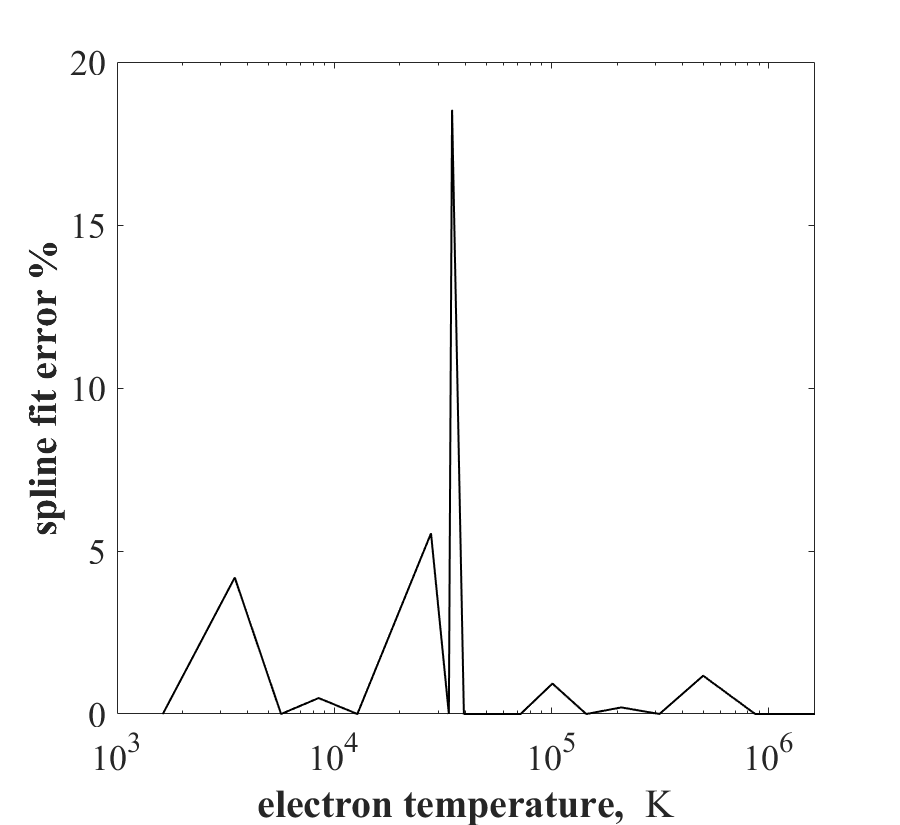
\includegraphics[width=0.99\linewidth, angle=0.0,scale=0.49]{electronimpact_figs/electronimpact_figure2_error.png}}
\caption{$E/N$ results for $\rm O_2$, showing (a) reduced electric field as a function of the electron temperature and (b) error percentage when fitting a cubic spline through the data. Experimental $\rm O_2$ data points are taken from \citen{book:1997:grigoriev}.}
\label{fig:electronimpact_2}
\end{figure}


%
\subsection{Nitric oxide ($\rm NO$)}

The results for NO are obtained by fitting a spline through BOLSIG+ and known experimental data. For electron temperatures less than 1000 K, the reduced electric field is computed assuming that the corresponding electron energy loss function $\zeta_{\rm e} $ in the local approximation takes the floor value of 0.001 according to the following equation:
%
\begin{equation}
\zeta_{\rm e}   =    \frac{2 m_{\rm e} \mu_{\rm e} N}{3  k_{\rm B} T_{\rm e} } \left[  \mu_{\rm e}N  \left(E/N(T_{\rm e})\right)^2\right]
\end{equation}
%
The final curve fit is shown in Fig. \ref{fig:electronimpact_3} alongside all the reference data used to obtain it. All the processes involving cross-sections used in the BOLSIG+ calculation are given in Table \ref{tab:tableNO}.

\begin{table*}[!htbp]
  \center\fontsizetable
  \begin{threeparttable}
    \tablecaption{$\rm NO$ electron impact processes with available cross-section data.}
    \label{tab:tableNO}
    \fontsizetable
    \begin{tabular*}{\textwidth}{l@{\extracolsep{\fill}}llll}
    \toprule
    {no.}  & {process} & {type} &  {eV range}  &  {ref.} \\
    \midrule
      1 & $\rm e^- + NO \rightarrow NO^+ + e^- + e^-$  &  ionization   &  9.26-1000 &   \cite{lxc:2024:morgan} \\ 
      \midrule     
      2 & $\rm e^- + NO \rightarrow e^- + NO$  &  momentum transfer   &  0.0-100  & \cite{lxc:2024:morgan}\\   
      \midrule
      3 & $\rm e^- + NO \rightarrow e^- + NO$$(\nu_1) $  &  vibrational excitation   &  0.30-100 & \cite{lxc:2024:morgan}\\ 
      4 & $\rm e^- + NO \rightarrow e^- + NO$$(\nu_2) $  &  vibrational excitation   &  0.45-100 & \cite{lxc:2024:morgan}\\ 
      5 & $\rm e^- + NO \rightarrow e^- + NO$$(\nu_3) $  &  vibrational excitation   &  0.75-100 & \cite{lxc:2024:morgan}\\ 
      6 & $\rm e^- + NO \rightarrow e^- + NO$$(\nu_4) $  &  vibrational excitation   &  0.90-100 & \cite{lxc:2024:morgan}\\ 
      7 & $\rm e^- + NO \rightarrow e^- + NO$$(\nu_5) $  &  vibrational excitation   &  1.20-100 & \cite{lxc:2024:morgan}\\ 
      8 & $\rm e^- + NO \rightarrow e^- + NO$$(\nu_6) $  &  vibrational excitation   &  1.35-100 & \cite{lxc:2024:morgan}\\ 
     \midrule
      9 & $\rm e^- + NO \rightarrow e^- + NO^* $  &  electronic excitation   &  5.50-100 & \cite{lxc:2024:morgan}\\ 
     10 & $\rm e^- + NO \rightarrow e^- + NO^* $  &  electronic excitation   &  6.60-100 & \cite{lxc:2024:morgan}\\
     11 & $\rm e^- + NO \rightarrow e^- + NO^* $  &  electronic excitation   &  9.26-100 & \cite{lxc:2024:morgan}\\
    \bottomrule
    \end{tabular*}
   \end{threeparttable}
\end{table*}

\begin{figure}[!htbp]
\subfigure[]{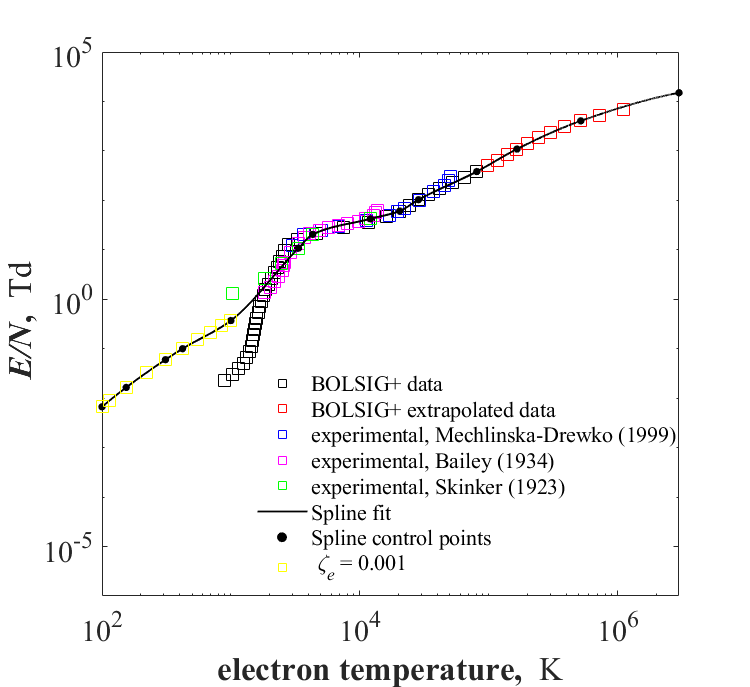
\includegraphics[width=0.99\linewidth, angle=0.0,scale=0.49]{electronimpact_figs/electronimpact_figure3.png}}
\subfigure[]{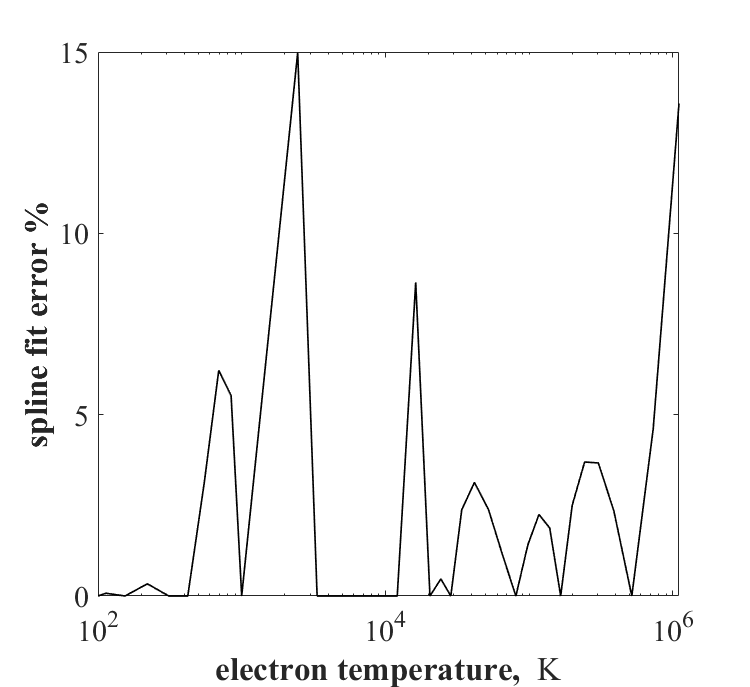
\includegraphics[width=0.99\linewidth, angle=0.0,scale=0.49]{electronimpact_figs/electronimpact_figure3_error.png}}
\caption{$E/N$ results for $\rm NO$, showing (a) reduced electric field as a function of the electron temperature and (b) error percentage when fitting a cubic spline through the data. Experimental data points are taken from Fig.\ 2 of Ref.\ \citen{jop:1999:mechlinska}, Fig.\ 5 of Ref.\ \citen{jos:1934:bailey} and Fig.\ 1.32 of Ref.\ \citen{jos:1934:skinker}. For electron temperatures less than 1000 K, the $E/N$ values are estimated by assuming a value of electron energy loss function $\zeta_{\rm e} = 0.001$. }
\label{fig:electronimpact_3}
\end{figure}
%
All the processes involving cross-sections used in the BOLSIG+ calculation are given in Table \ref{tab:tableNH3}. The reduced electric field results are shown in Fig. \ref{fig:electronimpact_3}.
%
\subsection{Ammonia ($\rm NH_3$)}

All the processes involving cross-sections used in the BOLSIG+ calculation are given in Table \ref{tab:tableNH3}. The reduced electric field results are shown in Fig. \ref{fig:electronimpact_6}.

\begin{table*}[!htbp]
  \center\fontsizetable
  \begin{threeparttable}
    \tablecaption{$\rm NH_3$ electron impact processes with available cross-section data.}
    \label{tab:tableNH3}
    \fontsizetable
    \begin{tabular*}{\textwidth}{l@{\extracolsep{\fill}}llll}
    \toprule
    {no.}  & {process} & {type} &  {eV range}  &  {ref.} \\
    \midrule
      1 & $\rm e^- + NH_3 \rightarrow NH + H_2^+ + e^- + e^-$  &  ionization   &  10-1000 &  \cite{psst:2023:snoeckx} \\
      2 & $\rm e^- + NH_3 \rightarrow NH_3^+ + e^- + e^-$  &  ionization   &  10-1000  & \cite{psst:2023:snoeckx}\\
      3 & $\rm e^- + NH_3 \rightarrow NH_2 + H^+ + e^- + e^-$  &  ionization   &  20-1000   &\cite{psst:2023:snoeckx}\\
      4 & $\rm e^- + NH_3 \rightarrow NH_2^+ + H + e^- + e^-$  &  ionization   &  10-1000  & \cite{psst:2023:snoeckx}\\      
      5 & $\rm e^- + NH_3 \rightarrow N^+ + H_2 + H + e^- + e^-$  &  ionization   &  10-1000   &\cite{psst:2023:snoeckx}\\         
      6 & $\rm e^- + NH_3 \rightarrow NH^+ + H_2 +  e^- + e^-$  &  ionization   &  20-1000   &\cite{psst:2023:snoeckx}\\  
      \midrule     
      7 & $\rm e^- + NH_3 \rightarrow e^- + NH_3$  &  momentum transfer   &  0-4000  & \cite{lxc:2024:morgan}\\   
      \midrule
      8 & $\rm e^- + NH_3 \rightarrow e^- + NH_3(V2)$  &  electronic excitation   &  0.118-1000 & \cite{lxc:2024:morgan}\\ 
      9 & $\rm e^- + NH_3 \rightarrow e^- + NH_3(V4)$  &  electronic excitation   &  0.202-1000 &\cite{lxc:2024:morgan}\\  
      10 & $\rm e^- + NH_3 \rightarrow e^- + NH_3(V13)$  &  electronic excitation   &  0.420-1000 &\cite{lxc:2024:morgan}\\  
      11 & $\rm e^- + NH_3 \rightarrow e^- + NH_3(E1)$  &  electronic excitation   &  5.720-1000 &\cite{lxc:2024:morgan}\\ 
      12 & $\rm e^- + NH_3 \rightarrow e^- + NH_3(E2)$  &  electronic excitation   &  8.650-1000 &\cite{lxc:2024:morgan}\\ 
      \midrule
      13 & $\rm e^- + NH_3 \rightarrow e^- + NH_3(\nu_1)$  &  vibrational excitation   &  0.42-34 &\cite{psst:2023:snoeckx}\\  
      14 & $\rm e^- + NH_3 \rightarrow e^- + NH_3(\nu_2)$  &  vibrational excitation   &  0.12-32 &\cite{psst:2023:snoeckx}\\ 
      15 & $\rm e^- + NH_3 \rightarrow e^- + NH_3(\nu_3)$  &  vibrational excitation   &  0.45-35 &\cite{psst:2023:snoeckx}\\ 
      16 & $\rm e^- + NH_3 \rightarrow e^- + NH_3(\nu_4)$  &  vibrational excitation   &  0.21-35 &\cite{psst:2023:snoeckx}\\ 
      \midrule
      17 & $\rm e^- + NH_3 \rightarrow e^- + NH_3(00\rightarrow10)$  &  rotational excitation   &  0.01-30 & \cite{psst:2023:snoeckx}\\ 
      18 & $\rm e^- + NH_3 \rightarrow e^- + NH_3(00\rightarrow20)$  &  rotational excitation   &  0.01-30 &\cite{psst:2023:snoeckx}\\ 
      19 & $\rm e^- + NH_3 \rightarrow e^- + NH_3(00\rightarrow30)$  &  rotational excitation   &  0.01-30 &\cite{psst:2023:snoeckx}\\ 
      20 & $\rm e^- + NH_3 \rightarrow e^- + NH_3(00\rightarrow40)$  &  rotational excitation   &  0.01-30 &\cite{psst:2023:snoeckx}\\ 
      21 & $\rm e^- + NH_3 \rightarrow e^- + NH_3(00\rightarrow50)$  &  rotational excitation   &  0.01-30 &\cite{psst:2023:snoeckx}\\ 
    \bottomrule
    \end{tabular*}
   \end{threeparttable}
\end{table*}
%
\begin{figure}[!htbp]
\subfigure[]{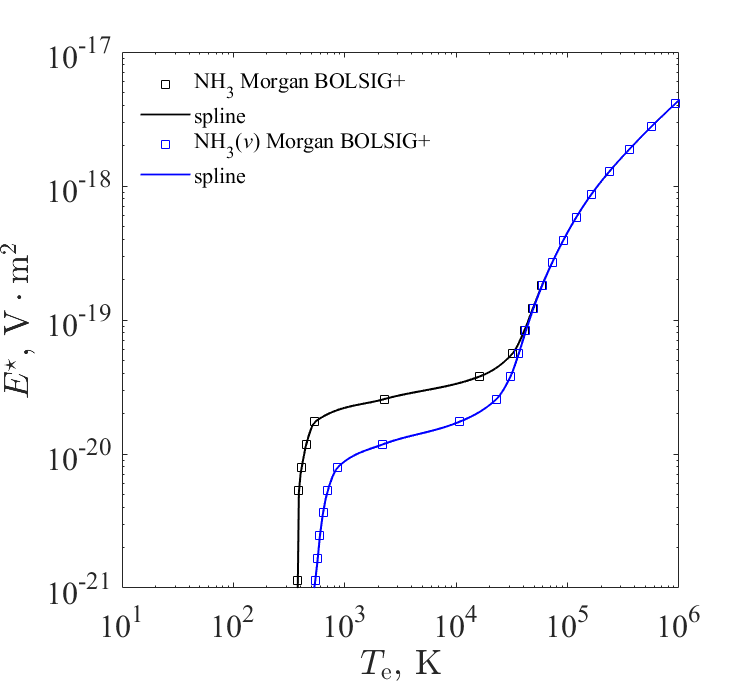
\includegraphics[width=0.99\linewidth, angle=0.0,scale=0.49]{electronimpact_figs/electronimpact_figure6.png}}
\subfigure[]{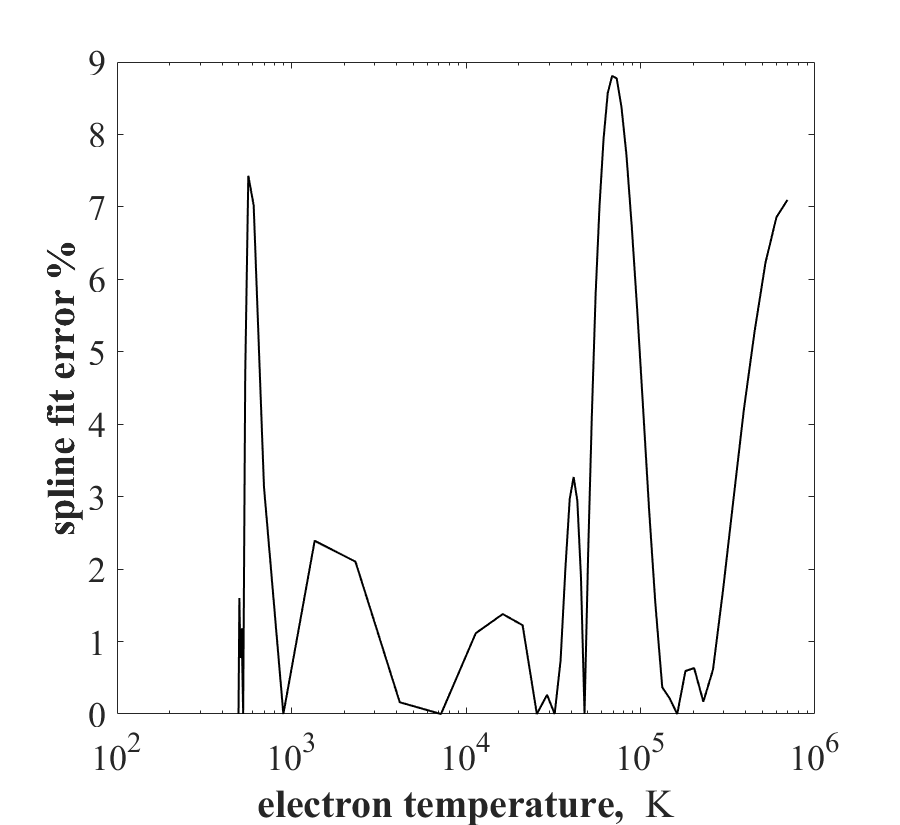
\includegraphics[width=0.99\linewidth, angle=0.0,scale=0.49]{electronimpact_figs/electronimpact_figure6_error.png}}
\caption{$E/N$ results for $\rm NH_3$, showing (a) reduced electric field as a function of the electron temperature and (b) error percentage when fitting a cubic spline through the data. The electron impact cross-sectional data used in the BOLSIG+ calculation is sourced from the Hayashi database, Ref.\ \cite{springer:1987:hayashi}.}
\label{fig:electronimpact_6}
\end{figure}
%


\begin{table}[!htbp]
  \center\fontsizetable
  \begin{threeparttable}
    \tablecaption{Coordinates of control points for monotone cubic spline interpolation of electron impact processes\tnote{a}.}
    \label{tab:spline_tab}
    \fontsizetable
    \begin{tabular*}{\textwidth}{l@{\extracolsep{\fill}}lcll}
    \toprule
   No.~~ & Process ~& Variable & Spline control point coordinates  \\
        \midrule

        

  \multirow{2}{*}{1} &  \multirow{2}{*}{ $\rm e^- + N  $   } & ${\rm ln}~T_{\rm e}$  & \tiny      6.1322    6.2124    6.4474    7.5872    8.7256    9.2774    9.4778    9.5934   10.0915   11.1390   11.7497   13.5255   15.4249
 \\
  &  & ${\rm ln}~E^\star$     & \tiny -55.2620  -54.4162  -53.5703  -51.4558  -49.7641  -48.9182  -48.0721  -47.2264  -45.1117  -43.4205  -42.5745  -40.8824  -39.6301\\     
  \midrule  
      
  \multirow{2}{*}{2} &  \multirow{2}{*}{ $\rm e^- + O  $   } & ${\rm ln}~T_{\rm e}$  & \tiny    6.1395    6.2392    6.5051    7.6315    8.6771    9.1363    9.2668    9.3848    9.5799   10.1629   10.8830   11.2996   11.6030   12.4065   15.4249 \\
  &  & ${\rm ln}~E^\star$     & \tiny  -55.2620  -54.4162  -53.5703  -51.4558  -49.7641  -48.9182  -48.0721  -47.2264  -46.3806  -45.1117  -44.2660  -43.4205  -42.5745  -40.8824  -39.0042\\     
  \midrule    
  
  \multirow{2}{*}{3} &  \multirow{2}{*}{ $\rm e^- + N_2 $   } & ${\rm ln}~T_{\rm e}$  & \tiny      5.7836    5.8854    6.0067    6.1891    7.0566    7.5266    7.7497    8.0862    8.8649    9.0580    9.1848    9.2866    9.5415    9.6956    9.7646   10.0010   10.6517   12.7964   15.4249
\\
  &  & ${\rm ln}~E^\star$     & \tiny     -51.8608  -51.3500  -51.0135  -50.6569  -49.5583  -49.0474  -48.7110  -48.3543  -47.2557  -46.7448  -46.4084  -46.0517  -44.9531  -44.4423  -44.1058  
 \\     
  &  &       & \tiny     -43.7491  -43.3907  -40.6829  -39.1439\\
  \midrule  
  
  \multirow{2}{*}{4} &  \multirow{2}{*}{ $\rm e^- + O_2  $   } & ${\rm ln}~T_{\rm e}$  & \tiny     5.6577    5.8861    6.4770    7.3930    8.1552    8.6458    9.0444    9.4545   10.2346   10.4239   11.1022   11.5585   15.4249
  \\
  &  & ${\rm ln}~E^\star$     & \tiny    -50.6569  -50.0691  -49.4041  -48.3543  -47.2557  -46.7448  -46.4084  -46.0517  -44.9531  -44.4423  -43.1821  -42.4533  -39.1439
  \\     
  \midrule  
  
  \multirow{2}{*}{5} &  \multirow{2}{*}{ $\rm e^- + NO  $   } & ${\rm ln}~T_{\rm e}$  & \tiny    4.6052    5.0387    5.7384    6.0438    6.9078    8.1163    8.3684    9.4004    9.9245   10.2589   11.3016   12.0194   13.1593   14.9141
 \\
  &  & ${\rm ln}~E^\star$     & \tiny    -53.3605  -52.4569  -51.1678  -50.6572  -49.3446  -45.9734  -45.3367  -44.6079  -44.2446  -43.7196  -42.4083  -41.3594  -40.0476  -38.7385
  \\     
  \midrule  
        
  \multirow{2}{*}{6} &  \multirow{2}{*}{ $\rm e^- + NH_3  $   } & ${\rm ln}~T_{\rm e}$  & \tiny 6.2086    6.2700    6.8003    8.8806   10.1453   10.3802   10.7743   11.9975   15.4249   \\
  
  &  & ${\rm ln}~E^\star$     & \tiny   -46.3062  -45.8896  -45.3691  -44.9524  -44.5359  -44.3277  -43.5990  -41.7243  -39.7238  \\
  
  
                       
    \bottomrule
    \end{tabular*}
\begin{tablenotes}
\item[{a}] Notation and units: $T_{\rm e}$ is the electron temperature in Kelvin and $E^\star$ is the reduced electric field in units of V$\rm ~m^2$.
\end{tablenotes}
   \end{threeparttable}
\end{table}








\appendix


  \bibliographystyle{warpdoc}
  \bibliography{all}


\end{document}







Old stuff

electron energy loss function: 
- not used anymore but kept just in case
- see derivation in prim/fluid/doc/Transport_Equations/report.pdf

%
\begin{table}
  \center\fontsizetable
  \begin{threeparttable}
    \tablecaption{Polynomial coefficients needed for the electron energy loss function $\zeta_{\rm e}=k_0+k_1 T_{\rm e}+k_2 T_{\rm e}^2 + k_3 T_{\rm e}^3 + k_4 T_{\rm e}^4 + k_5 T_{\rm e}^5+ k_6 T_{\rm e}^6$.\tnote{a,b,c}} 
    \label{tab:xicoefficients}
    \fontsizetable
    \begin{tabular}{llll}
    \toprule
      Coefficient & Value for $T_{\rm e}<19444$~K & Value for $T_{\rm e}\ge 19444$~K  \\
    \midrule
      $k_0$          & $+5.1572656\times 10^{-4}$ & $+2.1476152\times 10^{-1}$  \\
      $k_1$, 1/K     & $+3.4153708\times 10^{-8}$ & $-4.4507259\times 10^{-5}$  \\
      $k_2$, 1/K$^2$ & $-3.2100688\times 10^{-11}$ & $+3.5155106\times 10^{-9}$ \\
      $k_3$, 1/K$^3$ & $+1.0247332\times 10^{-14}$ & $-1.3270119\times 10^{-13}$ \\
      $k_4$, 1/K$^4$ & $-1.2153348\times 10^{-18}$ & $+2.6544932\times 10^{-18}$ \\
      $k_5$, 1/K$^5$ & $+7.2206246\times 10^{-23}$ & $-2.7145800\times 10^{-23}$ \\
      $k_6$, 1/K$^6$ & $-1.4498434\times 10^{-27}$ & $+1.1197905\times 10^{-28}$ \\
    \bottomrule
    \end{tabular}
 \begin{tablenotes}
   \item[a] The expression for $\zeta_{\rm e}$ can be used in the range $0<T_{\rm e}<60000$~K
   \item[b] In the range $287~{\rm K}<T_{\rm e}<1500$~K, the relative error that the loss function induces on the electron temperature is not more than 30\%.
   \item[c] In the range $1500~{\rm K}<T_{\rm e}<57000$~K, the relative error that the loss function induces on the electron temperature is not more than 5\%.
 \end{tablenotes}
   \end{threeparttable}
\end{table}
%


